\documentclass[a4paper,11pt]{report}
\usepackage[showexo=true,showcorr=false, showdegree=true]{../packages/coursclassed}
\usepackage{tikz}
\usetikzlibrary{calc}
\usetikzlibrary{positioning}
\usepackage{pgfplots}
\pgfplotsset{compat=1.15}
\usepackage{mathrsfs}
\usetikzlibrary{arrows}
\usepackage{pstricks-add}

\usepackage{tikz}

\newcount\segmentsleft
\tikzset{pics/.cd,
  circle fraction/.style args={#1/#2}{code={%
\segmentsleft=#1\relax
\pgfmathloop
\ifnum\segmentsleft<1\else
\ifnum\segmentsleft<#2 \edef\n{\the\segmentsleft}\else\def\n{#2}\fi
\begin{scope}[shift={(\pgfmathcounter*0.85,0)}]
\foreach \i [evaluate={\a=360/#2*(\i-1)+90;}] in {1,...,\n}
  \fill[fill=gray!70] (0,0) -- (\a:3/8) arc (\a:\a+360/#2:3/8) -- cycle;
\draw circle [radius=3/8];
\ifnum#2>1
  \foreach \i [evaluate={\a=360/#2*(\i-1);}] in {1,...,#2}
    \draw (0,0) -- (90+\a:3/8);
\fi
\end{scope}
\advance\segmentsleft by-#2
\repeatpgfmathloop
  }}
}




\toggletrue{montrerNiveaux}

\usepackage{enumitem}
\setlist[enumerate]{align=left,leftmargin=1cm,itemsep=10pt,parsep=0pt,topsep=0pt,rightmargin=0.5cm}
\setlist[itemize]{align=left,labelsep=1em,leftmargin=*,itemsep=0pt,parsep=0pt,topsep=0pt,rightmargin=0cm}

\setlength\columnsep{20pt}
\begin{document}

\newcommand{\chapterName}{Nombres et opérations}
\newcommand{\serieName}{Addition et soustraction de fractions}

\chapter*{\chapterName}
\thispagestyle{empty}

\begin{amL}{\serieName}{
\item Nombre rationnel (page 27)
\item Passer d'une écriture décimale finie à une écriture fractionnaire (page 28)
\item Amplification et simplification de fractions (page 29)
\item Additionner et soustraire des fractions (page 30)
}
\end{amL}
\section*{\serieName}
\setcounter{page}{1}


\begin{resolu}{Addition-Même dénominateur}{
Calcule et donne le résultat sous la forme d'une fraction irréductible ou d'un entier. 
\vspace{5pt}

\begin{tasks}
	\task  \begin{expli}
		\dfrac{1}{4}+\dfrac{1}{4}&=\dfrac{1+1}{4}& \text{Si (et seulement si!) les dénominateurs  sont}\\
				 && \text{égaux, on additionne les numérateurs.}\\
				 &=\dfrac{2}{4}&\text{On rend la fraction irréductible.}\\
				 \\
				&=\dfrac{1}{2}&\text{On donne le résultat sous la forme}\\
				&&\text{d'un entier ou d'une fraction irréductible.}
\end{expli}
\task \begin{expli}
		\dfrac{1}{3}+\dfrac{2}{3}&=\dfrac{1+2}{3}& \text{Si (et seulement si!) les dénominateurs  sont}\\
				 && \text{égaux, on additionne les numérateurs.}\\
				 &=\dfrac{3}{3}&\text{On rend la fraction irréductible.}\\
				 \\
				&=\dfrac{1}{1}&\text{On donne le résultat sous la forme}\\
				&=1&\text{d'un entier ou d'une fraction irréductible.}
\end{expli}
	\end{tasks}}{3}
\end{resolu}

\newpage
\begin{exo}
{Calcule et donne le résultat sous la forme d'une fraction irréductible ou d'un entier. 
\begin{tasks}(3)
\task $\dfrac{9}{11}+\dfrac{7}{11}= $ 
\task $\dfrac{4}{12}+\dfrac{5}{12}=$ 
\task $\dfrac{7}{18}+\dfrac{11}{18}=$
\task $\dfrac{5}{12}+\dfrac{13}{12}=$
\task $\dfrac{7}{9}+\dfrac{5}{9}=$
\task $\dfrac{1}{5}+\dfrac{9}{5}=$
\task $\dfrac{2}{13}+\dfrac{7}{13}=$
\task $\dfrac{8}{7}+\dfrac{6}{7}=$
\task $\dfrac{3}{4}+\dfrac{3}{4}=$
\task $\dfrac{2}{7}+\dfrac{5}{7}=$
\task $\dfrac{1}{3}+\dfrac{1}{3}=$
\task $\dfrac{1}{5}+\dfrac{3}{5}=$
\task  $\dfrac{5}{2}+\dfrac{3}{2}=$
\task   $\dfrac{2}{9}+\dfrac{5}{9}=$
\task $\dfrac{4}{6}+\dfrac{2}{6}=$
\end{tasks}
}{3}
\end{exo}

\begin{resolu}{Soustraction-Même dénominateur}{Calcule et donne le résultat sous la forme d'une fraction irréductible ou d'un entier. 
		\vspace{5pt}

\begin{tasks}
\task \begin{expli}
		\dfrac{3}{4}-\dfrac{1}{4}&=\dfrac{3-1}{4}& \text{Si (et seulement si!) les dénominateurs  sont}\\
				 && \text{égaux, on soustrait les numérateurs.}\\
				 &=\dfrac{2}{4}&\text{On rend la fraction irréductible.}\\
				 \\
				&=\dfrac{1}{2}&\text{On donne le résultat sous la forme}\\
				&&\text{d'un entier ou d'une fraction irréductible.}
\end{expli}
\task 
\begin{expli}
		\dfrac{4}{3}-\dfrac{1}{3}&=\dfrac{4-1}{3}& \text{Si (et seulement si!) les dénominateurs  sont}\\
				 && \text{égaux, on soustrait les numérateurs.}\\
				 &=\dfrac{3}{3}&\text{On rend la fraction irréductible.}\\
				 \\
				&=\dfrac{1}{1}&\text{On donne le résultat sous la forme}\\
				&=1&\text{d'un entier ou d'une fraction irréductible.}
\end{expli}
\task 
\begin{expli}
		\dfrac{7}{6}-\dfrac{3}{6}&=\dfrac{7-3}{6}& \text{Si (et seulement si!) les dénominateurs  sont}\\
				 && \text{égaux, on soustrait les numérateurs.}\\
				 &=\dfrac{4}{6}&\text{On rend la fraction irréductible.}\\
				 \\
				&=\dfrac{2}{3}&\text{On donne le résultat sous la forme}\\
				&&\text{d'un entier ou d'une fraction irréductible.}
\end{expli}
\end{tasks}
}
{3}
\end{resolu}
\begin{exo}
{Calcule ces différences et donne le résultat sous la forme d'une fraction irréductible ou d'un entier:
\begin{tasks}(3)
\task $\dfrac{4}{5}-\dfrac{1}{5}=$
\task $\dfrac{3}{9}-\dfrac{2}{9}=$
\task $\dfrac{7}{8}-\dfrac{2}{8}=$
\task $\dfrac{12}{7}-\dfrac{8}{7}=$
\task $\dfrac{17}{3}-\dfrac{8}{3}=$
\task $\dfrac{7}{2}-\dfrac{3}{2}=$
\task $\dfrac{9}{4}-\dfrac{6}{4}=$ 
\task $\dfrac{7}{3}-\dfrac{4}{3}=$
\task $\dfrac{8}{6}-\dfrac{2}{6}=$
\task $\dfrac{19}{8}-\dfrac{15}{8}=$
\task $\dfrac{27}{12}-\dfrac{1}{12}=$
\task $\dfrac{16}{16}-\dfrac{16}{16}=$
\end{tasks}
}{3}
\end{exo}

\begin{exo}
{Calcule et donne le résultat sous la forme d'une fraction irréductible ou d'un entier. 
\begin{tasks}(3)
\task $\dfrac{5}{6}+\dfrac{2}{6}= $ 
 \task $\dfrac{5}{7}-\dfrac{2}{7}=$ 
 \task $\dfrac{0}{5}+\dfrac{3}{5}=$
 \task $\dfrac{11}{8}+\dfrac{13}{8}=$
 \task $\dfrac{27}{12}-\dfrac{5}{12}=$
 \task $\dfrac{6}{50}-\dfrac{1}{50}=$
 \task $\dfrac{5}{6}+\dfrac{7}{6}=$
 \task $\dfrac{12}{19}-\dfrac{4}{19}=$\\ 
\end{tasks}
}{3}
\end{exo}

\begin{resolu}{Que reste-t-il de l'entier~?}{

Que reste-t-il de l'entier 1 si on enlève $\dfrac{1}{8}$~?

{\bfseries Solution:} On peut résoudre cet exercice de deux façons. La première en faisant un calcul:
\[1-\dfrac{1}{8}=\dfrac{8}{8}-\dfrac{1}{8}=\dfrac{7}{8}.\]

La deuxième en représentant graphiquement les fractions, la partie grisée représentant ce qu'on prend:
\begin{center}
			\scalebox{2.5}{
				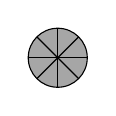
\begin{tikzpicture}[baseline={([yshift={-0.9\ht\strutbox}]current bounding box.north)}]
  %\node at (-1/2,0) {$\ldots\ldots\ldots$};
  \pic  at (0, 0) {circle fraction={8/8}};
\end{tikzpicture}-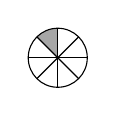
\begin{tikzpicture}[baseline={([yshift={-0.9\ht\strutbox}]current bounding box.north)}]

  %\node at (-1/2,0) {$\ldots\ldots\ldots$};
  \pic  at (0, 0) {circle fraction={1/8}};
\end{tikzpicture}=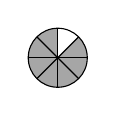
\begin{tikzpicture}[baseline={([yshift={-0.9\ht\strutbox}]current bounding box.north)}]

  %\node at (-1/2,0) {$\ldots\ldots\ldots$};
  \pic  at (0, 0) {circle fraction={7/8}};
\end{tikzpicture}}
\end{center}
}
{3}
\end{resolu}

\begin{exo}
{Que reste-t-il de l'entier 1 si l'on a enlève...~?
Représente graphiquement la fraction à l'aide d'un cercle ou d'un rectangle, puis donne la fraction restante.

\begin{tasks}(6)
\task $\dfrac{1}{3}$
\task $\dfrac{2}{5}$
\task $\dfrac{3}{8}$
\task $\dfrac{1}{2}$
\task $\dfrac{3}{4}$
\task $\dfrac{2}{7}$
\end{tasks}}
{3}
\end{exo}


\begin{resolu}{Additions et soustractions de fractions de dénominateurs différents  1/2}{Calcule et donne le résultat sous la forme d'une fraction irréductible ou d'un entier. 

\begin{tasks}
\task \begin{expli}
		\dfrac{1}{2}+\dfrac{1}{4}&=\dfrac{1\cdot 2}{2\cdot 2}+\dfrac{1}{4}& \text{Le }\operatorname{ppmc}(2;4)=4, \text{ donc on amplifie}\\
		      &&\text{par 2 la première fraction pour}\\	
		      &=\dfrac{2}{4}+\dfrac{1}{4}&\text{ avoir des dénominateurs égaux.}\\
		      &&\text{On additionne les fractions}\\
		      &=\dfrac{3}{4}&\text{comme vu précédemment.}\\

		      &&\text{On donne le résultat sous la forme}\\
				&&\text{d'un entier ou d'une fraction irréductible.}
\end{expli}
\task \begin{expli}
		\dfrac{1}{3}-\dfrac{1}{12}&=\dfrac{1\cdot 4}{3\cdot 4}-\dfrac{1}{12}& \text{Le }\operatorname{ppmc}(3;12)=12, \text{ donc on amplifie}\\
		      &&\text{par 4 la première fraction pour}\\	
		      &=\dfrac{4}{12}-\dfrac{1}{12}&\text{ avoir des dénominateurs égaux.}\\
		      &&\text{On additionne les fractions}\\
		      &=\dfrac{3}{12}&\text{comme vu précédemment.}\\

		      &&\text{On donne le résultat sous la forme}\\
		      &=\dfrac{1}{4}&\text{d'un entier ou d'une fraction irréductible.}
\end{expli}
\end{tasks}}
{3}
\end{resolu}

\begin{exop}
{Pour chacun des calcules suivants:
	\begin{enumerate}
    \item[1)] \text{Trouve le ppcm des deux dénominateurs.}
    \item[2)] \text{Complète les pointillés.}
    \item[3)] {\text Calcule et donne le résultat sous la forme d'une fraction irréductible ou d'un entier.}
\end{enumerate}
\vspace{5pt}

\begin{tasks}
	\task \[\dfrac{9}{4}+\dfrac{5}{12}=\dfrac{9\cdot\ldots\ldots}{4\cdot\ldots\ldots}+\dfrac{5}{12}=\dfrac{\ldots\ldots}{\ldots\ldots}\]
		\vspace{5pt}

		car $\operatorname{ppmc}(4;12)=\ldots\ldots$. 
	\task \[\dfrac{8}{5}-\dfrac{16}{10}=\dfrac{8\cdot\ldots\ldots}{5\cdot\ldots\ldots}-\dfrac{16}{10}=\dfrac{\ldots\ldots}{\ldots\ldots}\]
		\vspace{5pt}

	car $\operatorname{ppmc}(5;10)=\ldots\ldots$.
	\task \[\dfrac{5}{6}+\dfrac{5}{12}=\dfrac{5\cdot\ldots\ldots}{6\cdot\ldots\ldots}+\dfrac{5}{12}=\dfrac{\ldots\ldots}{\ldots\ldots}\]
		\vspace{5pt}

		car $\operatorname{ppmc}(6;12)=\ldots\ldots$.
	\task \[\dfrac{2}{3}-\dfrac{1}{18}=\dfrac{2\cdot\ldots\ldots}{3\cdot\ldots\ldots}-\dfrac{1}{18}=\dfrac{\ldots\ldots}{\ldots\ldots}\]
		\vspace{5pt}

	car $\operatorname{ppmc}(3;18)=\ldots\ldots$.
\end{tasks}}
{3}
\end{exop}

\begin{exo}
{Calcule et donne le résultat sous la forme d'une fraction irréductible ou d'un entier. 
\begin{tasks}(3)
\task $\dfrac{3}{5}+\dfrac{8}{10}=$
\task $\dfrac{2}{7}+\dfrac{1}{14}=$
\task $\dfrac{4}{15}+\dfrac{3}{5}=$
\task $\dfrac{5}{8}+\dfrac{1}{4}=$
\task $\dfrac{5}{6}+\dfrac{7}{12}=$
\task $\dfrac{2}{3}+\dfrac{3}{6}=$
\task $\dfrac{7}{15}+\dfrac{5}{3}=$
\task $\dfrac{3}{8}+\dfrac{5}{16}=$
\end{tasks}
}{3}
\end{exo}



\begin{exo}
{Calcule et donne le résultat sous la forme d'une fraction irréductible ou d'un entier. 

\begin{tasks}(3)
 \task $\dfrac{5}{6}+\dfrac{5}{12}=$
  \task $\dfrac{11}{3}-\dfrac{5}{6}=$
 \task $\dfrac{13}{14}+\dfrac{5}{7}=$
  \task $\dfrac{11}{9}-\dfrac{1}{3}=$  
  \task $\dfrac{3}{25}+\dfrac{2}{5}=$  
  \task $\dfrac{4}{3}-\dfrac{5}{21}=$  
\end{tasks}    
}{3}
\end{exo}

\begin{exo}
{Calcule et donne le résultat sous la forme d'une fraction irréductible ou d'un entier.

\begin{tasks}(3)
\task $\dfrac{1}{2}-\dfrac{1}{4}=$
\task $\dfrac{3}{2}-\dfrac{1}{8}=$
\task $\dfrac{3}{4}-\dfrac{3}{12}=$
\task $\dfrac{3}{6}-\dfrac{1}{2}=$
\task $\dfrac{3}{4}-\dfrac{5}{8}=$
\task $\dfrac{7}{8}-\dfrac{3}{4}=$
\end{tasks}}
{3}
\end{exo}

\begin{exo}
{Calcule et donne le résultat sous la forme d'une fraction irréductible ou d'un entier.

\begin{tasks}(3)
\task $\dfrac{2}{3}-\dfrac{1}{6}=$
\task $\dfrac{9}{10}-\dfrac{2}{5}=$
\task $\dfrac{3}{4}-\dfrac{7}{12}=$
\task $\dfrac{8}{9}-\dfrac{1}{3}=$
\task $\dfrac{7}{6}-\dfrac{5}{12}=$
\task $\dfrac{3}{5}-\dfrac{4}{15}=$
\end{tasks}}
{3}
\end{exo}


\begin{resolu}{Additions et soustractions de fractions de dénominateurs différents 2/2}{
Calcule et donne le résultat sous la forme d'une fraction irréductible ou d'un entier. 
\vspace{5pt}

\begin{tasks}
\task \begin{expli}
		\dfrac{11}{8}+\dfrac{5}{6}&=\dfrac{11\cdot 3}{8\cdot 3}+\dfrac{5\cdot 4}{6\cdot 4}& \text{Le }\operatorname{ppmc}(8;6)=24, \text{ on amplifie par 3}\\
		      &&\text{la première fraction et par 4 la deuxiÚme}\\	
		      &=\dfrac{33}{24}+\dfrac{20}{24}&\text{pour avoir des dénominateurs égaux.}\\
		      &&\text{On soustrait les fractions}\\
		      &=\dfrac{53}{24}&\text{comme vu précédemment.}\\

		      &&\text{On donne le résultat sous la forme}\\
		      &&\text{d'un entier ou d'une fraction irréductible.}
\end{expli}
\task \begin{expli}
		\dfrac{5}{9}-\dfrac{1}{4}&=\dfrac{5\cdot 4}{9\cdot 4}-\dfrac{1\cdot 9}{4\cdot 9}& \text{Le }\operatorname{ppmc}(9;4)=36, \text{ on amplifie par 4}\\
		      &&\text{la première fraction et par 9 la deuxiÚme}\\	
		      &=\dfrac{20}{36}-\dfrac{9}{36}&\text{pour avoir des dénominateurs égaux.}\\
		      &&\text{On soustrait les fractions}\\
		      &=\dfrac{11}{36}&\text{comme vu précédemment.}\\

		      &&\text{On donne le résultat sous la forme}\\
		      &&\text{d'un entier ou d'une fraction irréductible.}
\end{expli}
\end{tasks}}
{3}
\end{resolu}

\begin{exop}
{Pour chacun des calculs suivants:
	\begin{enumerate}
    \item[1)] \text{Trouve le ppcm des deux dénominateurs.}
    \item[2)] \text{Complète les pointillés.}
    \item[3)] {\text Calcule et donne le résultat sous la forme d'une fraction irréductible ou \\
    d'un entier.}
\end{enumerate}
\vspace{3pt}

\begin{tasks}
	\task \[\dfrac{5}{9}+\dfrac{7}{4}=\dfrac{5\cdot\ldots\ldots}{9\cdot\ldots\ldots}+\dfrac{7\cdot \ldots\ldots}{4\cdot \ldots\ldots}=\dfrac{\ldots\ldots}{\ldots\ldots}\]
		\vspace{3pt}

	car $\operatorname{ppmc}(9;4)=\ldots\ldots$.
	\task \[\dfrac{5}{3}-\dfrac{5}{4}=\dfrac{5\cdot\ldots\ldots}{3\cdot\ldots\ldots}-\dfrac{5\cdot \ldots\ldots}{4\cdot \ldots\ldots}=\dfrac{\ldots\ldots}{\ldots\ldots}\]
		\vspace{3pt}

	car $\operatorname{ppmc}(3;4)=\ldots\ldots$.
	\task \[\dfrac{2}{3}+\dfrac{8}{5}=\dfrac{2\cdot\ldots\ldots}{3\cdot\ldots\ldots}+\dfrac{8\cdot \ldots\ldots}{5\cdot \ldots\ldots}=\dfrac{\ldots\ldots}{\ldots\ldots}\]
		\vspace{3pt}

	car $\operatorname{ppmc}(3;5)=\ldots\ldots$.
	\task \[\dfrac{5}{10}-\dfrac{2}{15}=\dfrac{5\cdot\ldots\ldots}{10\cdot\ldots\ldots}-\dfrac{2\cdot \ldots\ldots}{15\cdot \ldots\ldots}=\dfrac{\ldots\ldots}{\ldots\ldots}\]
		\vspace{3pt}

	car $\operatorname{ppmc}(10;15)=\ldots\ldots$.
\end{tasks}}
{3}
\end{exop}
\begin{exol}{NO215}{56}{3}
\end{exol}
\begin{exol}{NO216}{57}{3}
\end{exol}
\begin{exof}{NO223}{76}{3}
\end{exof}


\begin{exo}
{Calcule et donne le résultat sous la forme d'une fraction irréductible ou d'un entier.
\begin{tasks}(3)
\task $\dfrac{2}{3}+\dfrac{6}{5}=$
\task $\dfrac{3}{2}-\dfrac{1}{3}=$
\task $\dfrac{7}{3}-\dfrac{3}{2}=$
\task $\dfrac{13}{52}-\dfrac{1}{20}=$
\task $\dfrac{5}{9}+\dfrac{2}{18}=$
\task $\dfrac{5}{6}+\dfrac{2}{8}=$
\end{tasks}    
}{3}
\end{exo}

\begin{exo}
{Calcule et donne le résultat sous la forme d'une fraction irréductible ou d'un entier.
\begin{tasks}(3)
\task $\dfrac{3}{4}+\dfrac{5}{7}=$
\task $\dfrac{13}{14}-\dfrac{1}{4}=$
\task $\dfrac{5}{11}-\dfrac{2}{33}=$
\task $\dfrac{6}{12}+\dfrac{3}{36}=$
\task $\dfrac{3}{9}+\dfrac{2}{18}=$
\task $\dfrac{6}{24}+\dfrac{3}{4}=$
\end{tasks}    
}{3}
\end{exo}


\begin{resolu}{Fraction et entier}{
Calcule et donne le résultat sous la forme d'une fraction irréductible ou d'un entier. 
\vspace{5pt}

\begin{tasks}
\task 
\begin{expli}
	1+\dfrac{1}{4}&=\dfrac{1}{1}+\dfrac{1}{4}& \text{On passe en écriture fractionnaire.}\\
		      &&\text{On amplifie pour avoir des}\\	
		      &=\dfrac{1\cdot 4}{1 \cdot 4}+\dfrac{1}{4}&\text{dénominateurs égaux.}\\
		      &&\text{On additionne les fractions}\\
		      &=\dfrac{4}{4}+\dfrac{1}{4}&\text{comme vu prcédemment.}\\

		      &&\text{On donne le résultat sous la forme}\\
				&=\dfrac{5}{4}&\text{d'un entier ou d'une fraction irréductible.}
\end{expli}

\task \begin{expli}
	2-\dfrac{1}{6}&=\dfrac{2}{1}-\dfrac{1}{6}& \text{On passe en écriture fractionnaire.}\\
		      &&\text{On amplifie pour avoir des}\\	
		      &=\dfrac{2\cdot 6}{1 \cdot 6}+\dfrac{1}{6}&\text{dénominateurs égaux.}\\
		      &&\text{On soustrait les fractions}\\
		      &=\dfrac{12}{6}-\dfrac{1}{6}&\text{comme vu précédemment.}\\

				&&\text{On donne le résultat sous la forme}\\
				&=\dfrac{11}{6}&\text{d'un entier ou d'une fraction irréductible.}
\end{expli}
\end{tasks}}
{3}
\end{resolu}

\begin{exo}
{Complète les pointillés, puis calcule et donne le résultat sous la forme d'une fraction irréductible ou d'un entier. 
\begin{tasks}(2)
\task $1+\dfrac{2}{6}= \dfrac{1\cdot\ldots}{1\cdot\ldots}+ \dfrac{2}{6}= $ 
\task $2+\dfrac{1}{3}=\dfrac{2\cdot\ldots}{1\cdot\ldots}+ \dfrac{1}{3}=$ 
\task $\dfrac{16}{3}+3=\dfrac{16}{3}+\dfrac{3\cdot\ldots}{1\cdot\ldots}=$
\task $\dfrac{3}{4}+2=\dfrac{3}{4}+\dfrac{2\cdot\ldots}{1\cdot\ldots}=$
\end{tasks}
}{3}
\end{exo}

\begin{exo}
{Complète les pointillés, puis calcule et donne le résultat sous la forme d'une fraction irréductible ou d'un entier. 
\begin{tasks}(2)
\medskip\task $1-\dfrac{2}{6}= \dfrac{1\cdot\ldots}{1\cdot\ldots}- \dfrac{2}{6}=$ 
\medskip \task $2-\dfrac{1}{3}=\dfrac{2\cdot\ldots}{1\cdot\ldots}- \dfrac{1}{3}=$ 
\medskip \task $\dfrac{16}{3}-3= \dfrac{16}{3}-\dfrac{3\cdot\ldots}{1\cdot\ldots}=$ 
\medskip \task $\dfrac{13}{4}-2=\dfrac{13}{4}-\dfrac{2\cdot\ldots}{1\cdot\ldots}=$
\end{tasks}
}{3}
\end{exo}

\begin{exo}
{Calcule et donne le résultat sous la forme d'une fraction irréductible ou d'un entier. 
\begin{tasks}(3)
\task $4-\dfrac{3}{2}= $ 
 \task $2+\dfrac{1}{4}=$ 
 \task $\dfrac{9}{4}-1=$
 \task $4+\dfrac{5}{7}=$
 \task $\dfrac{16}{3}-3=$
 \task $2+\dfrac{3}{4}=$ 
\end{tasks}
}{3}
\end{exo}

\begin{exop}
{Complète les pointillés  par un nombre entier:	
\begin{tasks}(3)
\task $\dfrac{4}{6}+\dfrac{\ldots\ldots\ldots}{6}=1$
\task $\dfrac{2}{3}+\dfrac{\ldots\ldots\ldots}{3}=1$

\task $\dfrac{4}{9}+\dfrac{\ldots\ldots\ldots}{\ldots\ldots\ldots}=1$
\task $\dfrac{7}{8}+\dfrac{\ldots\ldots\ldots}{\ldots\ldots\ldots}=1$
\task $\dfrac{4}{5}+\dfrac{\ldots\ldots\ldots}{5}=1$
\task $\dfrac{81}{83}+\dfrac{\ldots\ldots\ldots}{\ldots\ldots\ldots}=1$
\end{tasks}
}{3}
\end{exop}

\begin{resolu}{Fractions et décimaux}{Calcule et donne le résultat sous la forme d'une fraction irréductible ou d'un entier. 
		\vspace{5pt}

\begin{tasks}
\task \begin{expli}
		\dfrac{7}{5}+7,5&=\dfrac{7}{5}+\dfrac{75}{10}& \text{On passe en écriture fractionnaire.}\\
		      &&\text{On amplifie pour avoir des}\\	
		      &=\dfrac{7\cdot 2}{5\cdot 2}+\dfrac{75}{10}&\text{dénominateurs égaux.}\\
		      &&\text{On additionne les fractions}\\
		      &=\dfrac{14}{10}+\dfrac{75}{10}&\text{comme vu précédemment.}\\

		      &&\text{On donne le résultat sous la forme}\\
				&=\dfrac{89}{10}&\text{d'un entier ou d'une fraction irréductible.}
\end{expli}

\task \begin{expli}
		\dfrac{11}{8}+1,25&=\dfrac{11}{8}+\dfrac{125}{100}& \text{On passe en écriture fractionnaire.}\\
		      &&\text{On amplifie pour avoir des}\\	
		      &=\dfrac{11\cdot 25}{8 \cdot 25}+\dfrac{125\cdot 2}{100\cdot 2}&\text{dénominateurs égaux.}\\
		      &&\text{On additionne les fractions}\\
		      &=\dfrac{275}{200}+\dfrac{250}{200}&\text{comme vu précédemment.}\\
		      &&\text{On donne le résultat sous }\\
		      &=\dfrac{525}{200}&\text{la forme d'un entier ou}\\
		      &&\text{d'une fraction irréductible.}\\
				&=\dfrac{21}{8}&
\end{expli}
\end{tasks}}
{3}
\end{resolu}

\begin{exop}
{Pour chacun des calculs suivants:
	\begin{enumerate}
    \item[1)] Transforme le nombre décimal en une fraction décimale.
    \item[2)] Trouve le ppmc des deux dénominateurs.
    \item[3)] Complète les pointillés.
    \item[4)] Calcule et donne le résultat sous la forme d'une fraction irréductible ou d'un entier.
\end{enumerate}
\vspace{5pt}

\begin{tasks}
	\task \[\dfrac{13}{6}-1,5=\dfrac{13}{6}-\dfrac{\ldots\ldots}{\ldots\ldots}=\dfrac{13\cdot \ldots\ldots}{6\cdot \ldots\ldots}-\dfrac{\ldots\ldots}{\ldots\ldots}=\dfrac{\ldots\ldots}{\ldots\ldots}\]
\vspace{5pt}

		car $\operatorname{ppmc}(6;\ldots\ldots)=\ldots\ldots$.

	\task \[1,2+\dfrac{3}{5}=\dfrac{\ldots\ldots}{\ldots\ldots}+\dfrac{3}{5}=\dfrac{\ldots\ldots}{\ldots\ldots}+\dfrac{3\cdot \ldots\ldots}{5\cdot \ldots\ldots}=\dfrac{\ldots\ldots}{\ldots\ldots}\]
\vspace{5pt}

		car $\operatorname{ppmc}(\ldots\ldots;5)=\ldots\ldots$.
	\task \[0,5+1,75=\dfrac{\ldots\ldots}{\ldots\ldots}+\dfrac{\ldots\ldots}{\ldots\ldots}=\dfrac{\ldots\ldots}{\ldots\ldots}+\dfrac{\ldots\ldots}{\ldots\ldots}=\dfrac{\ldots\ldots}{\ldots\ldots}\]
\vspace{5pt}

		car $\operatorname{ppmc}(\ldots\ldots;\ldots\ldots)=\ldots\ldots$.
\end{tasks}}
{3}
\end{exop}


\begin{exol}{NO217}{57}{3}
\end{exol}
\begin{exol}{NO218}{58}{3}
\end{exol}

\begin{exo}
 {Calcule et donne le résultat sous la forme d'une fraction irréductible ou d'un entier.
	 \begin{tasks}(2)
\task $\dfrac{2}{3}+0,5=$
\task $\dfrac{13}{5}-1,5=$
\task $4,5-\dfrac{1}{4}=$
\task $7,35-\dfrac{3}{5}=$
\end{tasks}}
{3}
\end{exo}

\begin{resolu}{Fractions et périodiques}{Voici une liste de fractions utiles:
		\begin{tasks}(2)
    \task $\dfrac{1}{3}=0,\overline{3} $
    \task $\dfrac{2}{3}=0,\overline{6} $
    \task $\dfrac{1}{9}=0,\overline{1}$
    \task $\dfrac{1}{7}=0,\overline{142857}$
\end{tasks}

Calcule et donne le résultat sous la forme d'une fraction irréductible ou d'un entier. 

\begin{tasks}(2)
    \task $\dfrac{1}{2}+0,\overline{3}=\dfrac{1}{2}+ \dfrac{1}{3}=\dfrac{5}{6}$
   \task $0,\overline{6}+\dfrac{1}{3}=\dfrac{2}{3}+\dfrac{1}{3}=\dfrac{3}{3}=1$
\end{tasks}}
{3}
\end{resolu}

\begin{exo}
{Calcule et donne le résultat sous la forme d'une fraction irréductible ou d'un entier.

	\begin{tasks}(2)
\task $\dfrac{8}{9}-0,\overline{6}=$
\task$\dfrac{1}{2}-0,\overline{3}=$
\task $\dfrac{4}{9}+4,\overline{3}=$
\task $\dfrac{1}{4}+1,\overline{6}=$
\end{tasks}}
{3}
\end{exo}

\begin{exo}
 {Calcule et donne le résultat sous la forme d'une fraction irréductible ou d'un entier.

	 \begin{tasks}(2)
\task $\dfrac{5}{8}+17,05=$
\task$0,5-0,\overline{3}=$
\task $ 3,45+0,\overline{3}=$
\task $\dfrac{1}{8}+3,\overline{6}=$
\end{tasks}
}
{3}
\end{exo}

\begin{exo}
 {Calcule et donne le résultat sous la forme d'une fraction irréductible ou d'un entier.
\begin{tasks}(3)
 \task  $\dfrac{5}{3}+2-\dfrac{3}{4}=$
 \task  $\dfrac{7}{8}+2,5+\dfrac{1}{16}=$
 \task $3,6-\dfrac{1}{3}=$
 \task  $0,025+2-\dfrac{1}{3}=$
 \task  $\dfrac{2}{3}+\dfrac{3}{4}-1=$
 \task $0,6-\dfrac{1}{3}=$
\end{tasks}
}{3}
\end{exo}



\begin{exol}{NO219}{58}{3}
\end{exol}
\begin{exof}{NO220}{75}{3}
\end{exof}
\begin{exof}{NO221}{75}{3}
\end{exof}

\begin{exo}
{Calcule et donne le résultat sous la forme d'une fraction irréductible ou d'un entier.
	\begin{tasks}(2)
\task $\dfrac{1}{2}+\dfrac{5}{12}+0,\overline{3}=$
\task $30,05+\dfrac{2}{5}=$
\task $\dfrac{4}{7}-0,\overline{3}=$
\task $0,05+\dfrac{1}{4}+0,\overline{6}=$
\task $5+\dfrac{2}{11}=$
\task $9,2-1,\overline{3}=\phantom{\dfrac{1}{5}}$
\end{tasks}}
{3}
\end{exo}

\begin{exof}{NO222}{76}{3}
\end{exof}
\begin{exo}
{Complètes les pointillés par un entier.

\begin{tasks}(2)
\task  $\dfrac{4}{5}+\dfrac{\ldots}{\ldots}=\dfrac{21}{20}$
\task $\dfrac{2}{3}+3=\dfrac{\ldots}{\ldots}$
\task $1,\overline{3}-\dfrac{\ldots}{\ldots}=0,5$
\task  $\dfrac{13}{52}-\dfrac{8}{20}=\dfrac{\ldots}{\ldots}$
\task  $1,\overline{6}+0,\overline{3}=\dfrac{\ldots}{\ldots}\phantom{\dfrac{1}{2}}$
\task $\dfrac{6}{3}-\dfrac{\ldots}{\ldots}=\dfrac{7}{6}$
\end{tasks}
}
{3}
\end{exo}

\begin{exo}
{J'ai mangé un quart, puis deux tiers d'un gâteau. 
\begin{enumerate}
    \item Quelle fraction du gâteau ai-je mangé~?
    \item Quelle fraction du gâteau reste-t-il~?
\end{enumerate}}
{3}
\end{exo}


\begin{exo}
{Marc a dépensé $\dfrac{1}{4}$ de son argent de poche pour s'acheter une BD et $\dfrac{2}{3}$ pour acheter un cadeau à sa soeur.


\begin{enumerate}
    \item Quelle fraction de son argent a-t-il dépensé~?
    \item Quelle fraction lui reste-t-t-il~?
\end{enumerate}}
{3}
\end{exo}

\begin{exo}
{J'ai passé le $\dfrac{3}{7}$ de mes vacances en Italie et les $\dfrac{2}{14}$ chez mes grands-parents. Le reste, je les passe tranquillement chez moi.

\begin{enumerate}
    \item Quelle fraction de mes vacances ai-je passé hors de chez moi~?
    \item Quelle fraction lme reste-til chez moi~?
\end{enumerate}}
{3}
\end{exo}

\begin{exol}{NO235}{61}{3}
\end{exol}

\begin{exol}{NO223}{58}{3}
\end{exol}

\begin{exol}{NO226}{59}{3}
\end{exol}

\begin{exol}{NO229}{60}{3}
\end{exol}

\begin{exol}{NO231}{60}{3}
\end{exol}

\begin{exol}{NO238}{62}{3}
\end{exol}


\end{document}
